%% abtex2-modelo-trabalho-academico.tex, v-1.9.2 laurocesar
%% Copyright 2012-2014 by abnTeX2 group at http://abntex2.googlecode.com/ 
%%
%% This work may be distributed and/or modified under the
%% conditions of the LaTeX Project Public License, either version 1.3
%% of this license or (at your option) any later version.
%% The latest version of this license is in
%%   http://www.latex-project.org/lppl.txt
%% and version 1.3 or later is part of all distributions of LaTeX
%% version 2005/12/01 or later.
%%
%% This work has the LPPL maintenance status `maintained'.
%% 
%% The Current Maintainer of this work is the abnTeX2 team, led
%% by Lauro César Araujo. Further information are available on 
%% http://abntex2.googleco@misc{MarileneCarneiroMatos,

%%
%% This work consists of the files abntex2-modelo-trabalho-academico.tex,
%% abntex2-modelo-include-comandos and abntex2-modelo-references.bib
%%
% ------------------------------------------------------------------------
% ------------------------------------------------------------------------
% abnTeX2: Modelo de Trabalho Academico (tese de doutorado, dissertacao de
% mestrado e trabalhos monograficos em geral) em conformidade com 
% ABNT NBR 14724:2011: Informacao e documentacao - Trabalhos academicos -
% Apresentacao
% ------------------------------------------------------------------------
% ------------------------------------------------------------------------

\documentclass[
	% -- opções da classe memoir --
	12pt,				% tamanho da fonte
	openright,			% capítulos começam em pág ímpar (insere página vazia caso preciso)
	oneside,			% para impressão em verso e anverso. Oposto a oneside
	a4paper,			% tamanho do papel. 
	% -- opções da classe abntex2 --
	%chapter=TITLE,		% títulos de capítulos convertidos em letras maiúsculas
	%section=TITLE,		% títulos de seções convertidos em letras maiúsculas
	%subsection=TITLE,	% títulos de subseções convertidos em letras maiúsculas
	%subsubsection=TITLE,% títulos de subsubseções convertidos em letras maiúsculas
	% -- opções do pacote babel --
	english,			% idioma adicional para hifenização
	brazil				% o último idioma é o principal do documento
	]{abntex2}

% ---
% Pacotes básicos 
% ---
\usepackage{unitins}
\usepackage{lmodern}			% Usa a fonte Latin Modern			
\usepackage[T1]{fontenc}		% Selecao de codigos de fonte.
\usepackage[utf8]{inputenc}		% Codificacao do documento (conversão automática dos acentos)
\usepackage{lastpage}			% Usado pela Ficha catalográfica
\usepackage{indentfirst}		% Indenta o primeiro parágrafo de cada seção.
\usepackage{color}				% Controle das cores

\usepackage{graphicx}			% Inclusão de gráficos
\usepackage{subfig}
\usepackage{microtype} 			% para melhorias de justificação
\usepackage{soul}
\usepackage{amssymb}
\usepackage{amsmath}
\usepackage{spreadtab}
\usepackage{multirow}
\usepackage{amsthm}
\usepackage{url}
\usepackage{siunitx}

%Adicionado para criar Matrizes, cases e layouts no latex
\usepackage{array}
\usepackage{mathdots}

\usepackage{float}

\usepackage[portuguese, ruled, linesnumbered]{algorithm2e}


\usepackage{algorithmic}

% Utilizado para customizar as fontes das equações 
\usepackage{fixmath}
\usepackage{verbatim}

% ---
		
% ---
% Pacotes adicionais, usados apenas no âmbito do Modelo Canônico do abnteX2
% ---
		% para geração de dummy text
% ---

% ---
% Pacotes de citações
% ---


%\usepackage[brazilian,hyperpageref]{backref}	 % Paginas com as citações na bibl
\usepackage[alf,abnt-etal-list=2,abnt-repeated-author-omit=yes]{abntex2cite}	% Citações padrão ABNT

\usepackage{multirow}
\usepackage[table,xcdraw]{xcolor}
\usepackage{colortbl}
\definecolor{lightgray}{gray}{0.9}
\graphicspath{{imagens/}}

%INCLUDE PDF 

\usepackage{pdfpages}

% LONG TABLE - TABELA LONGA 

%\usepackage[margin=1in]{geometry}
\usepackage{longtable,tabularx,ltxtable}

\usepackage{threeparttablex} % for "ThreePartTable" environment
\usepackage{pgfplotstable}
\usepackage{filecontents}
\usepackage{makecell}
\usepackage{booktabs}
\usepackage{float}

\usepackage[brazil]{babel} % for European Portuguese use portuguese
\usepackage[fixlanguage]{babelbib}
\selectbiblanguage{brazil}
\citeoption{abnt-etal-cite=2}


\usepackage[running]{lineno}

% \newcolumntype{Y}{>{\centering\arraybackslash}X}
%\setlength\LTleft{0pt}
%\setlength\LTright{0pt}

%\usepackage[justification=centering]{caption}

% \theoremstyle{theorem}
%\newtheorem{theorem}{Theorem}
%\newtheorem{teo}{Teorema}[chapter]
%\newtheorem{lema}[teo]{Lema}
%\theoremstyle{definition}
%\newtheorem{defi}[teo]{Definição}

% --- 
% CONFIGURAÇÕES DE PACOTES
% --- 

% ---
% Configurações do pacote backref
% Usado sem a opção hyperpageref de backref
%\renewcommand{\backrefpagesname}{Citado na(s) página(s):~}
% Texto padrão antes do número das páginas
%\renewcommand{\backref}{}
% Define os textos da citação
%\renewcommand*{\backrefalt}[4]{
%	\ifcase #1 %
%		Nenhuma citação no texto.%
%	\or
%		Citado na página #2.%
%	\else
%		Citado #1 vezes nas páginas #2.%
%	\fi}%
% ---

% ---
% Informações de dados para CAPA e FOLHA DE ROSTO
% ---
\titulo{Desenvolvimento de uma biblioteca para o monitoramento de ruídos em dados
coletados de sensores embarcados}
\autor{Tales Monteiro Melquiades}
\local{Palmas}
\data{2021}
\orientador{Prof. Me. Marco Antonio Firmino De Sousa}
\instituicao{%
  Universidade Estadual do Tocantins
  \par
  Curso de Sistemas de Informação
  }
\tipotrabalho{Projeto de conclusão de curso (Graduação)}
% O preambulo deve conter o tipo do trabalho, o objetivo, 
% o nome da instituição e a área de concentração 
\preambulo{Projeto apresentado como requisito para aprovação
na disciplina de Trabalho de conclusão de Curso de
Sistemas de Informações da Universidade Estadual
do Tocantins - UNITINS, sob a Orientação do Prof.
Me. Marco Antonio Firmino De Sousa.}

% ---


% ---
% Configurações de aparência do PDF final

% alterando o aspecto da cor azul
\definecolor{blue}{RGB}{41,5,195}

% informações do PDF
\makeatletter
\hypersetup{
     	%pagebackref=true,
		pdftitle={\@title}, 
		pdfauthor={\@author},
    	pdfsubject={\imprimirpreambulo},
		%pdfcreator={LaTeX with abnTeX2},
		pdfkeywords={Algoritmo}{trabalho acadêmico}, 
		colorlinks=true,       		% false: boxed links; true: colored links
    	linkcolor=blue,          	% color of internal links
    	citecolor=blue,        		% color of links to bibliography
    	filecolor=magenta,      		% color of file links
		urlcolor=blue,
		bookmarksdepth=4
}
\makeatother
% --- 

% --- 
% Espaçamentos entre linhas e parágrafos 
% --- 

% O tamanho do parágrafo é dado por:
\setlength{\parindent}{1.3cm}

% Controle do espaçamento entre um parágrafo e outro:
\setlength{\parskip}{0.2cm}  % tente também \onelineskip

% ---
% compila o indice
% ---
\makeindex
% ---

% ----
% Início do documento
% ----
\begin{document}

% Retira espaço extra obsoleto entre as frases.
\frenchspacing

% ----------------------------------------------------------
% ELEMENTOS PRÉ-TEXTUAIS
% ----------------------------------------------------------
% \pretextual
% ----------------------------------------------------------

% ----------------------------------------------------------
% ELEMENTOS PRÉ-TEXTUAIS
% ----------------------------------------------------------
% \pretextual

% ---
% Capa
% ---
\imprimircapa
% ---

% ---
% Folha de rosto
% (o * indica que haverá a ficha bibliográfica)
% ---
\imprimirfolhaderosto
% ---

% ---
% Inserir folha de aprovação
% ---

% Isto é um exemplo de Folha de aprovação, elemento obrigatório da NBR
% 14724/2011 (seção 4.2.1.3). Você pode utilizar este modelo até a aprovação
% do trabalho. Após isso, substitua todo o conteúdo deste arquivo por uma
% imagem da página assinada pela banca com o comando abaixo:
%
% \includepdf{folhadeaprovacao_final.pdf}
%
\begin{folhadeaprovacao}



	\begin{center}
		
\includegraphics[width=1\textwidth]{imagens/unitins.png}
		\ABNTEXchapterfont\Large   CURSO DE SISTEMAS DE INFORMA{\c{C}}{\~{A}}O

		\par
		\vspace*{1cm}
		{\ABNTEXchapterfont\bfseries\large \expandafter\MakeUppercase{\imprimirtitulo}  \vspace*{1cm}    }
		\par
		{\large \expandafter\MakeUppercase{\imprimirautor}}
		%\vspace*{\fill}
		\par
		\vspace*{1cm}
		\hspace{.45\textwidth}
		\begin{minipage}{.5\textwidth}
			\small\imprimirpreambulo

		\end{minipage}%
		%	\vspace*{\fill}
	\end{center}



	\assinatura{\textbf{\imprimirorientador} \\ Orientador}
	\assinatura{\textbf{Professor} \\ Convidado 1}
	\assinatura{\textbf{Professor} \\ Convidado 2}
	%\assinatura{\textbf{Professor} \\ Convidado 3}
	%\assinatura{\textbf{Professor} \\ Convidado 4}

	\begin{center}
		\vspace*{0.5cm}
		{\large\imprimirlocal}
		\par
		{\large\imprimirdata}
		\vspace*{1cm}
	\end{center}

\end{folhadeaprovacao}
% ---

% ---
% Dedicatória
% ---
\begin{dedicatoria}
	\vspace*{\fill}
	\centering
	\noindent
	\textit{A todas as pessoas que direta ou indiretamente contribuíram para a realização deste trabalho.} \vspace*{\fill}
\end{dedicatoria}
% ---

% ---
% Agradecimentos
% --- Es
\begin{agradecimentos}
	Ao meu orientador, pelo suporte no pouco tempo que lhe coube, pelas suas correções e incentivos.
	Agradeço a todos os  meus professores por me proporcionar o conhecimento e afetividade da educação 
	no processo de formação profissional, pela excelência da qualidade técnica de cada um.
	Aos meus pais que sempre me incentivaram a superar as dificuldades.
	Aos meus amigos de jornada, por não me deixarem desistir.
	A todos que direta ou indiretamente fizeram parte de minha formação, o meu muito obrigado.


\end{agradecimentos}
% ---

% ---
% Epígrafe
% ---
\begin{epigrafe}
	\vspace*{\fill}
	\begin{flushright}
		\textit{``The way to the stars is open.''\\
			Sergei Korolev}
	\end{flushright}
\end{epigrafe}
% ---

% ---
% RESUMOS
% ---

% resumo em português
\setlength{\absparsep}{18pt} % ajusta o espaçamento dos parágrafos do resumo
\begin{resumo}
	A leitura de dados vindos de sensores em tempo real sempre foi uma tarefa difícil e custosa. Há uma grande quantidade de ruído proveniente da baixa qualidade dos sensores e sequelas resultantes do ambiente, que produzem uma imensa quantidade de dados imprecisos e incorretos, estes os quais atrapalham na tomada de decisão de sistemas embarcados. 
	Neste trabalho foi implementado uma função de intervalo de confiança móvel, que pode ser utilizada em conjunto com outros métodos para obter dados mais precisos sem interferir no resultado final, o código tem como objetivo trabalhar de forma amigável em ambiente de sistema embarcado onde memória e processamento são recursos escassos e valiosos. Os resultados mostraram que o intervalo de confiança pode ser utilizado em certas ocasiões onde o tempo de espera não é tão custoso, retornando dados sempre dentro de um padrão aceitável de leitura mas perdendo qualidade na leitura de grandes curvas.


	% O problema é muito estudado pela comunidade científica, diversos trabalhos apontam diferentes formas de tratar e ignorar ruídos advindos de sensores. Notou-se a grande presença de artigos recentes que aprofundam o assunto em diversas áreas do conhecimento onde a leitura de dados tem um papel crítico e decisivo no resultado final, os quais são tratados e apresentados aqui com uma revisão bibliométrica que apresenta uma visão dos termos, artigos e autores dos últimos 5 anos desde a concepção deste trabalho. 
	
	% Neste trabalho também foi implementado funções de filtro populares e uma função de filtragem probabilística, em um repositório de código aberto apelidado de zscilib, focado em um conjunto de funções úteis para computação científica, análise de dados e manipulação de dados no contexto de dispositivos de hardware embarcado, desenvolvido especialmente para o sistema operacional de tempo real Zephyr mantido pela fundação Linux. As contribuições aqui propostas serão integradas a comunidade de código aberto e servirão para que outros pesquisadores, estudantes e atuantes da área possam usufruir e contribuir com a implementação código proposto.



	\textbf{Palavras-chaves}: Algoritmo de filtragem, Sistemas embarcados, Software, Sensor, Redução de ruído.
\end{resumo}

% resumo em inglês
\begin{resumo}[Abstract]
	\begin{otherlanguage*}{english}
		Reading data from sensors in real time has always been a difficult and costly task. There is a large amount of noise from the low quality of the sensors and consequences resulting from the environment, which produce a huge amount of inaccurate and incorrect data, which hinder decision-making in embedded systems.
		In this work, a mobile confidence interval function was implemented, which can be used in conjunction with other methods to obtain more accurate data without interfering with the final result, the code aims to work in a friendly way in an embedded system environment where memory and processing they are scarce and valuable resources. The results showed that the confidence interval can be used in certain occasions where the waiting time is not so costly, always returning data within an acceptable reading pattern but losing quality when reading large curves.
		\vspace{\onelineskip}

		\noindent
		\textbf{Key-words}: Filtering algorithm, Embedded systems, Software, Sensor, Noise reduction.
	\end{otherlanguage*}
\end{resumo}


% ---
% inserir lista de ilustrações
% ---
\pdfbookmark[0]{\listfigurename}{lof}
\listoffigures*
% ---

% ---
% inserir lista de tabelas
% ---
\newpage
\pdfbookmark[0]{\listtablename}{lot}
\newpage
\listoftables*
\cleardoublepage
% ---

% ---
% inserir lista de abreviaturas e siglas
% ---
\begin{siglas}
	\item RTOS - Sistema operacional de tempo-real.
	\item ISR - Rotinas de serviço de interrupção.
	\item SO - Sistema operacional.
	\item IC - Intervalo de confiança.
	\item SRAM - Memória Estática de Acesso Aleatório
	\item ROM - Memória de somente leitura
\end{siglas}
% ---


% ---
% inserir o sumario
% ---
\pdfbookmark[0]{\contentsname}{toc}
\tableofcontents*
\cleardoublepage
% ---



% ELEMENTOS TEXTUAIS
% ---------------------------------[!htb]-------------------------
%\textual

%Capitulos
% ----------------------------------------------------------
% Introdução (exemplo de capítulo sem numeração, mas presente no Sumário)
% ----------------------------------------------------------

\chapter{Introdução}\label{intro}
\section{Conceitos Introdutórios e Problematização}

O mundo moderno é cercado por sensores passivos que coletam dados de praticamente tudo, para monitoramento ou tomada de decisão, a maioria desses dispositivos é bombardeada de interferências indesejáveis o tempo todo. Seja pela baixa qualidade dos equipamentos ou pela grande quantidade de intervenções aleatórias de fontes externas que podem prejudicar o resultado final.

Umas das abordagens mais populares para escapar de valores discrepantes, e a utilização do cálculo de média móvel ou média móvel ponderada para remover ruídos, no entanto essa abordagem não apresenta uma boa eficiência energética e demanda muito tempo para conseguir refletir mudanças bruscas no dataset utilizado \cite{International_Conference__Zhuang}. 
Os dados ruidosos se caracterizam como leituras perdidas dos sensores ou leituras imprecisas e não confiáveis, dificultando o trabalho das aplicações que tentam usar os valores colhidos em sua forma original \cite{Jeffery_Pipelined_Framework}, com isso quase todas as aplicações que tentam ser confiáveis utilizam algum tipo de algoritmo de filtragem de dados advindos de sensores eletrônicos.
Os sensores modernos são construídos de forma a serem pequenos, baratos e eficientes energeticamente, para que possam ser utilizados em todos os lugares de forma massiva e descartável, consequentemente a qualidade não é eficiente o suficiente para não apresentar problemas com interferências \cite{tan2005sensoclean}. 


O método de média interfere nos valores finais alterando ou não conseguindo acompanhar em tempo real características importantíssimas como picos e alterações bruscas no valor, é importante que o método de filtragem distorça o mínimo possível principalmente se tratar de dados que irão participar de tomadas de decisões importantes, outro principal problema na filtragem de dados e a falta de um critério quantitativo da qualidade do filtro \cite{kalambet2011noise}.





\section{Objetivos e Escopo de Pesquisa}
\subsection{Objetivos de Pesquisa}
O trabalho aqui proposto se dispõe em testar o método de intervalo de confiança, como uma alternativa aos métodos tradicionais para obtenção de dados provindos de sensores sem interferência de ruídos, visto a exorbitante quantidade de dados provindo de sensores, somando a incerteza da qualidade de fabricação dos componentes eletrônicos de baixo custo disponíveis em ampla quantidade no mercado, com dados coletados de sensores conectados ao kit de desenvolvimento ESP32 v1 com o sistema operacional de tempo real \cite{Zephyr}.

% Com isso em mente o trabalho aqui proposto se dispõem de construir uma biblioteca de código aberto, que disponibilizara funções adequadas para a filtragem de dados provindo de sensores em ambiente de tempo real com multitarefas, testando a coleta e filtragem de dados no processador dual core ESP32 no sistema operacional de tempo real \cite{Zephyr}.

\subsection{Objetivos secundários}
Os objetivos secundários a serem alcançados são:
\begin{itemize}
\item Realizar uma revisão bibliométrica de trabalhos que utilizam de métodos probabilísticos para filtragem de dados de sensores;
\item Avaliar a utilização do método aqui proposto como uma alternativa aos métodos de média móvel e média móvel ponderada;
% \item Disponibilizar o código de forma aberta a comunidade, para que possa ser utilizado por qualquer outro interessado em tratar dados de sensores em ambiente de multitarefas 
\item Escrever funções de filtragem utilizando os métodos de Desvio padrão e Intervalo de confiança.
\end{itemize}


\section{Justificativa}
Dados provindos do mundo real são constantemente contaminados com ruídos ou podem não corresponder à realidade, esse tipo de situação pode afetar perigosamente um programa de computador qualquer que lida com dados de sensores. Muitos programas podem depender que essa resposta deva ser rápida o suficiente para não comprometer o desempenho e a segurança do programa, um veículo autômato ou um equipamento médico por exemplo não podem trabalhar com dados incorretos, mesmo que sejam em curtos períodos de tempo, os mesmos dependem que a resposta vinda dos sensores sejam rápidas e verdadeiras, com as respostas discrepantes sendo descartadas não comprometendo sua missão. 

Assim, em um primeiro momento considerou-se desenvolver e testar uma função de intervalo de confiança móvel para a filtragem de dados indesejáveis vindo de sensores diversos em tempo real, tendo como característica atuar de forma amigável junto a um RTOS sobre o microprocessador ESP32 da fabricante Espressif, em conjunto com o RTOS Zephyr um projeto mantido pela Linux Foundation.
% Assim então este trabalho visa contribuir com a construção de uma biblioteca na linguagem C é de código aberto, onde será oferecido funções para tratamento de dados ruidosos advindos do mundo real, cuidando de se preocupar em trabalhar em conjunto com o RTOS Zephyr, economizando tempo de desenvolvimento e centralizando código aberto para todo e qualquer projetista de software interessado em consumir e contribuir ao projeto.


\section{Organização do Trabalho}
Este trabalho está organizado da seguinte forma, para o capítulo 1 apresentou-se a introdução da pesquisa, com dados e justificativas baseadas na bibliografia de suas áreas, contendo também os objetivos do trabalho, além do escopo e justificativas. Já no capítulo 2 apresenta-se uma revisão bibliométrica acerca dos trabalhos relacionados e do escopo deste projeto. O capítulo 3 contém aspectos da metodologia adotada e os requisitos necessários, com o  capítulo 4 
% TODO: Inserir mudanças para projeto novo
possuindo os resultados obtidos detalhadamente, que por último contendo o capítulo 5 traz as conclusões retiradas desta pesquisa, com suas possíveis contribuições e benefícios para a sociedade, comunidade científica e de desenvolvimento em sistemas embarcados.
 

% Texto corrido
% ---
% Capitulo de revisão de literatura
% ---


\chapter{Trabalhos Relacionados}\label{referencial_teorico}
Aqui será dedicado a descrever os trabalhos relacionados, descrevendo cada um dos estudos 
e abordando seus pontos fortes e fracos. O autor \cite{Garcia} define uma serie de estrategias 
para avaliar um RTOS moderno, passando por diversos pontos importantes em um sistema de tempo real, 
como resposta a eventos externos, compartilhamento de recurso e sincronização entre tarefas. 
Em \cite{Raymundo} o autor se baseia nestas estrategias, 
implementando com novas tecnicas em 5 sistemas operacionais diferentes, inclusive nos dois 
sistemas propostos aqui neste trabalho, seu trabalho tem um foque em internet das coisas, 
tendo como base a plataforma de hardware NXP/Freescale FRDM-K64F.
No estudo \cite{nicolas2019avaliaccao}, o autor busca compreender e avaliar o funcionamento 
do FreeRTOS embarcado em um cubesat real, o estudo explica o funcionamento do sistema em 
cada um de seus pontos como, controle e escalonamento de tarefas, gerenciamento de filas e 
meemória, erros comuns e etc. Para avaliar o sistema, o mesmo foca numa serie de experimentos 
que são voltados ao funcionamento do sistema em um ambiente real de operação, tendo como vista 
problemas relacionados a radiação, perca de memória, corrompimento de dados e estouro de memória.
Os trabalhos trabalhos de \cite{Garcia} e \cite{Raymundo} tem foque nas qualidades do sistema, já 
o trabalho de \cite{nicolas2019avaliaccao} foca no desenpelho do sistema em ambiente real, perante 
a problemas externos e de missão.

\chapter{Revisão Bibliométrica sobre CubeSats e Zephyr RTOS}\label{referencial_teorico}

Nesta seção são consideradas informações referentes á produção acadêmica mundial, que 
abordam os temas Zephyr RTOS, CubeSats e Sistemas Operacionais de tempo real aplicados 
em plataformas de Nano-Satélites e CubeSats, foi realizada uma revisão bibliométrica 
sobre estes temas. 


Com a miniaturização e industrialização de componentes eletrônicos antes inacessíveis 
público comum, permitiu-se que diversas missões espaciais pudessem ser elaboradas rapidamente 
e com um baixo custo de produção, levando ao desenvolvimento de satélites menores que passaram 
não somente de ferramentas educacionais, mas para uma plataforma padrão de tecnologia e 
instrumentação científica \cite{Selva2012}. Estas plataformas construídas com componentes de 
prateleira (COTS) desenvolvidas em forma de cubo, possibilitam pesquisas científicas já cada 
vez mais reconhecidas com recursos de instrumentação que foram aplicadas em satélites maiores, 
promovendo a pesquisa em ambiente espacial antes restrito a grande agentes, agora a 
universidades e países em desenvolvimento \cite{Woellert2011}.


A Figura~\ref{fig: CubeSat NanoSatC-Br2} mostra o um dos CubeSats desenvolvido no Brasil pela Universidade 
Federal de Santa Maria (UFSM) com apoio da Agência Espacial Brasileira (AEB), Ministério de Ciência e 
Tecnologia (MCTI) e do Instituto Nacional de Pesquisas Espaciais (INPE).

\begin{figure}[H]
	\centering
	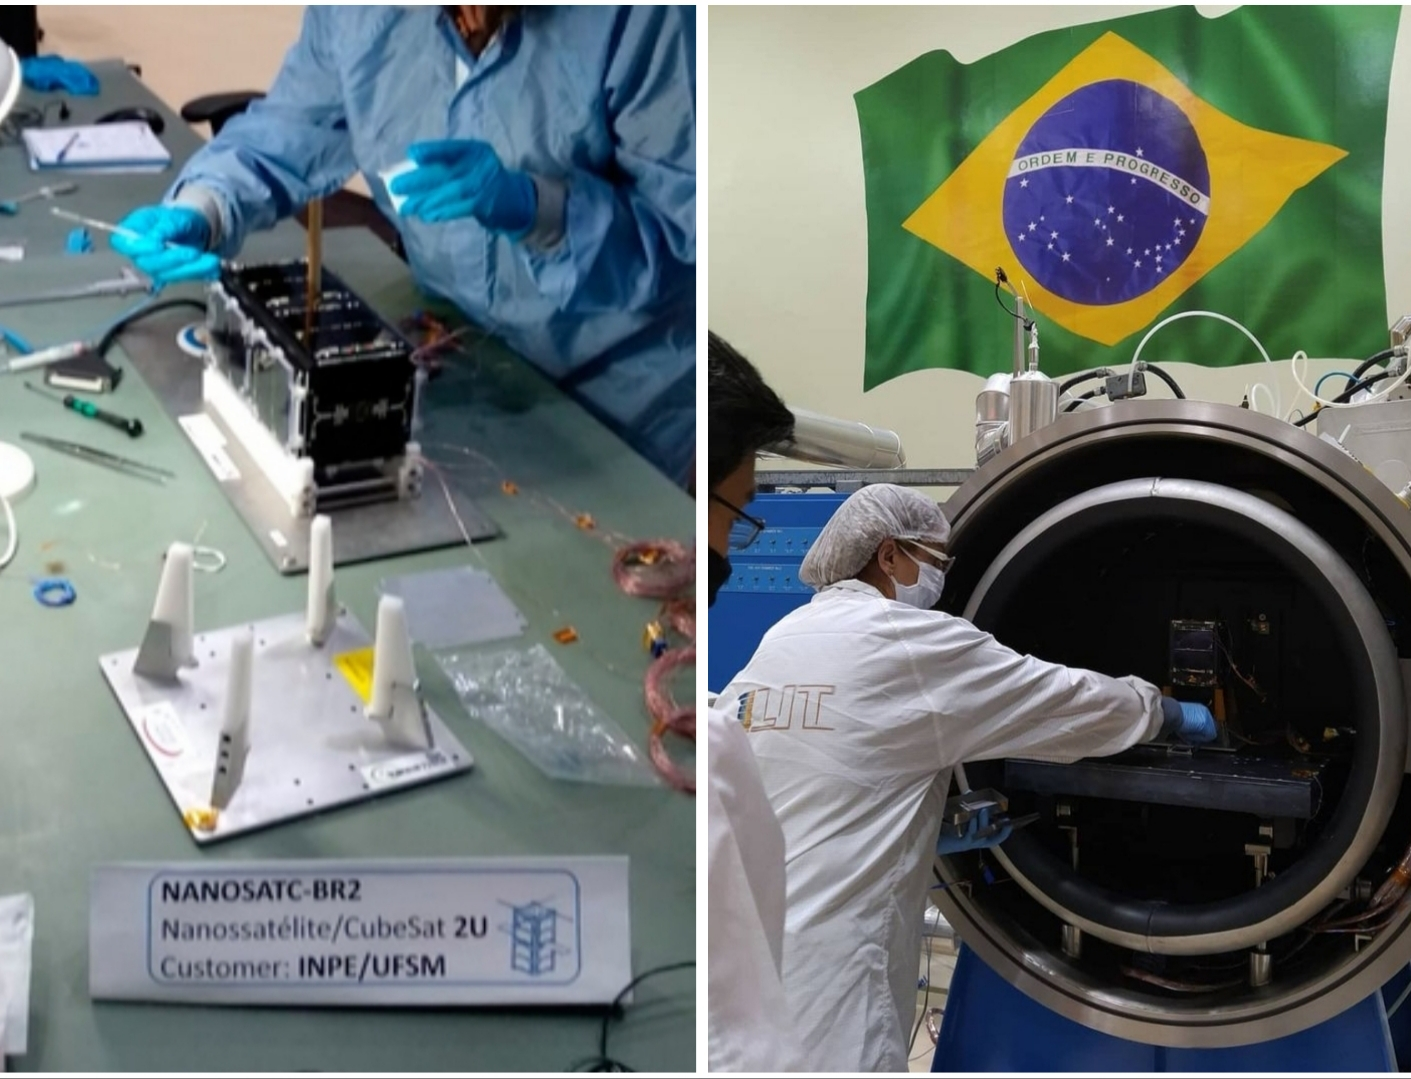
\includegraphics[width=15cm]{imagens/cubesat_brasil.jpg}
	\caption{NanoSatC-Br2 durante o processo de integração e teste no LIT/INPE}
	Fonte: Portal "www.tecnoveste.com.br", Lançamento de mais um satélite brasileiro – NanoSatC-Br2.
	\label{fig: CubeSat NanoSatC-Br2}
\end{figure}

\subsection{Zephyr RTOS}
Há mais de 20 anos nascia o primeiro RTOS do mercado, desde então outros sistemas tem trazido 
contribuições para o mundo embarcado. Um sistema operacional de tempo real se difere de um sistema 
operacional comum por depender diretamente do momento em que a ação foi produzida, buscando 
manter o tempo de mudança de contexto mínimo e gerenciando a execução de tarefas de acordo com 
suas prioridades \cite{Hambarde}. Os aplicativos de tempo real se tornaram populares devido a 
complexidade dos sistemas modernos, paralelo a isso o mercado de RTOS é bastante grande, com 
diversos antagonistas fornecendo ferramentas para resolver problemas de tempo real em diversas 
plataformas e de diversas maneiras, tornando a escolha cada vez mais difícil \cite{Hambarde}.


Zephyr é um RTOS de código aberto gerido pela Linux Foundation, construído sobre recursos
limitados e pensado em segurança e proteção, frequentemente adotado em sistemas críticos \cite{Zhao}.
Suportando uma grande variedade de placas de hardware e utilizado por empresas como Google, Intel
e Facebook. Oferece cooperatividade e segmentação preemptiva, alocação estática de memória,
isolamento de thread e dispositivos de proteção de memória \cite{nyffenegger2020connecting}.

\begin{figure}[H]
	\centering
	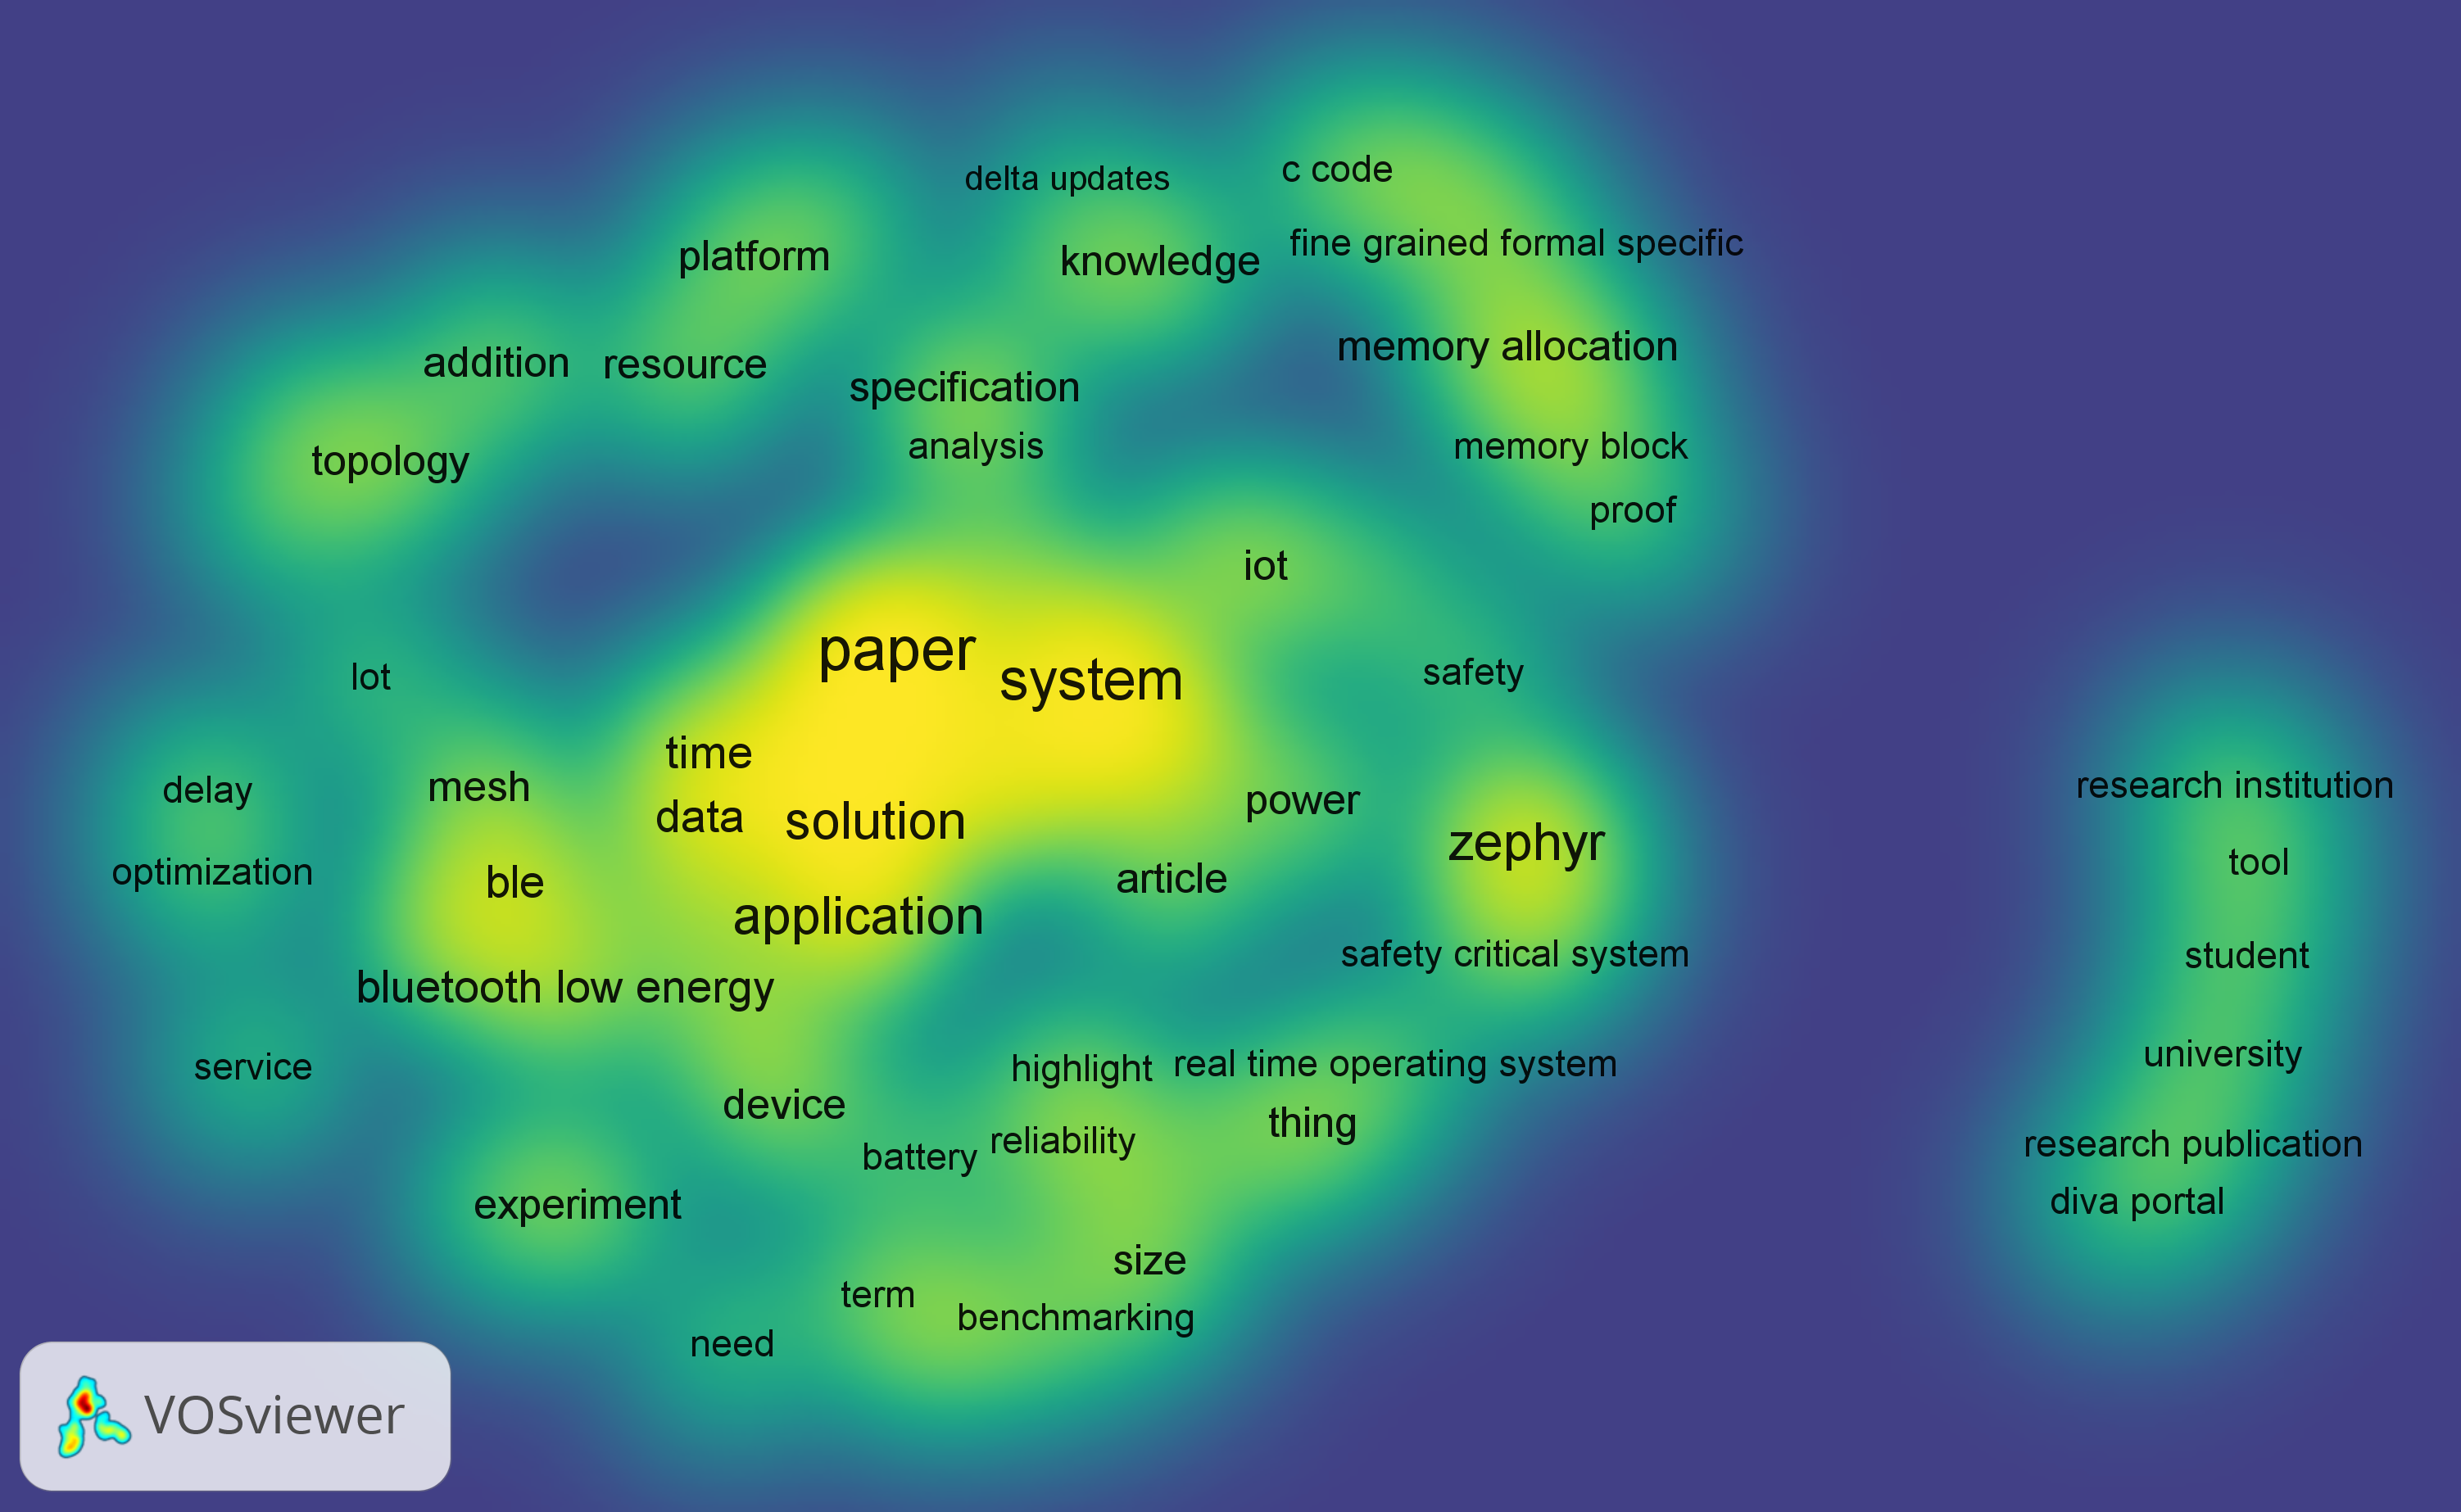
\includegraphics[width=15cm]{imagens/Zephyr_RTOS_Density_Visualization.png}
	\caption{Mapa de visualização de densidade sobre o termo "Zephyr RTOS"}
	Fonte: Autor com base no Software VOSViwer.
	\label{fig: Zephyr Density Visualization}
\end{figure}

A Figura~\ref{fig: Zephyr Density Visualization} representa uma espécie de "mapa de calor" sobre o 
tema "Zephyr RTOS" no mecanismo de busca Google Scholar, ao seu redor pode-se notar termos que 
remetem a RTOS como "safety critical system", "iot", "bluetooth low energy" e "memory allocation". 
Também e possível notar os termos "solution", "application", "service" e "plataform" que reforçam a 
ideia de que zephyr é amplamente utilizada em diversas plataformas e projetos\cite{nyffenegger2020connecting}.

\begin{figure}[H]
	\centering
	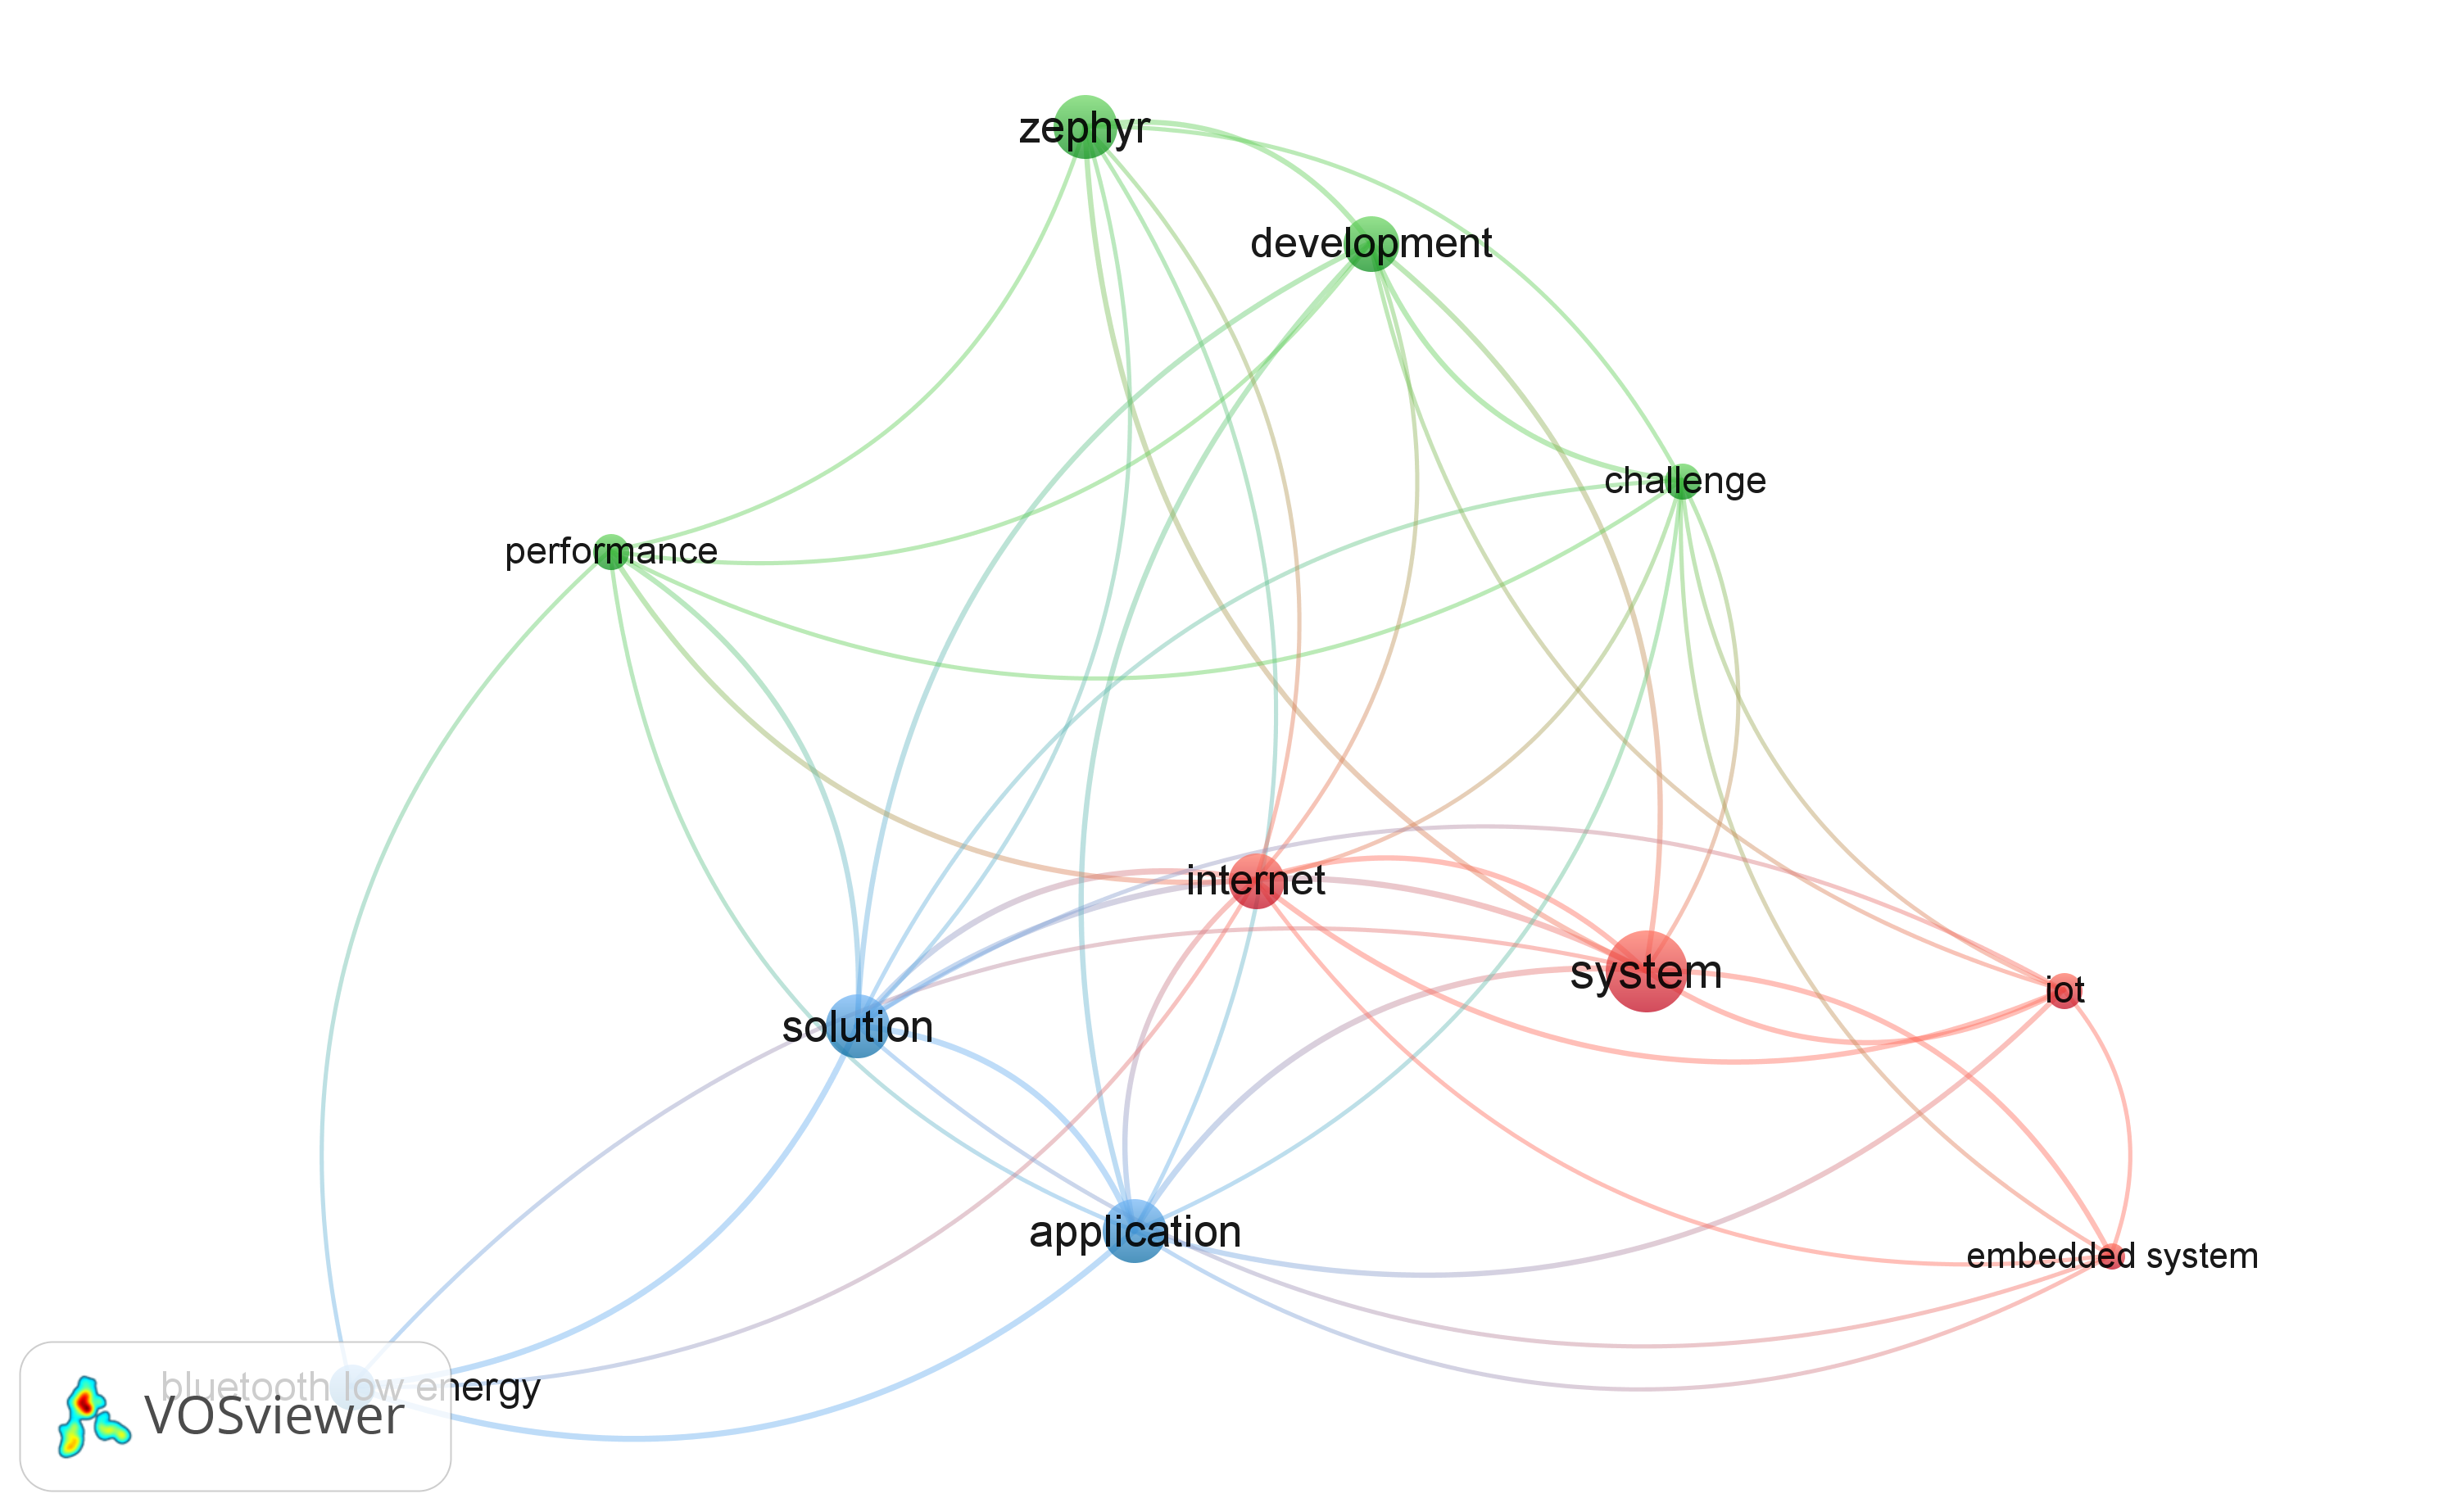
\includegraphics[width=15cm]{imagens/Zephyr_RTOS_Network_visualization.png}
	\caption{Mapa de visualização de rede sobre o termo "Zephyr RTOS"}
	Fonte: Autor com base no Software VOSViwer.
	\label{fig: Zephyr Network Visualization}
\end{figure}

A Figura~\ref{fig: Zephyr Network Visualization} demonstra uma rede de conexões entre o termo "Zephyr RTOS" 
e outros termos populares em sua pesquisa, nota-se conexões importantes entre zephyr e termos importante sem 
sua área. O tempo iot esta diretamente ligado a sistemas embarcados, sendo ligado ao zephyr através do termo 
"internet", o sistema é construído e mantido por diferentes empresas que trabalham no campo IOT 
\cite{huber_porting_2019}.


\subsection{Software CubeSat}
Para afunilar este estudo bibliométrico mais especifico para o termo central deste trabalho, realizou-se o 
levantamento sobre os termos "Cubesat SO", na base de trabalhos e citações Google Acadêmico, foi selecionado 
do período de 2012 a 2021 sendo encontrados aproximadamente 16.900 resultados, entre artigos, livros, 
citações e outros materiais acadêmicos. CubeSats são pequenos satélites limitados a cubos de 10cm³ atualmente 
muito populares, criado por Dr. Jordi Puig-Suari e Bob Twiggs, sendo uma espaçonave de custo e lançamento 
relativamente acessível \cite{Manyak2011FaultTA}. Na Figura~\ref{fig: Cubesat Density Visualization}nota-se 
os termos com mais destaques encontrados na busca feita neste trabalho.


\begin{figure}[H]
	\centering
	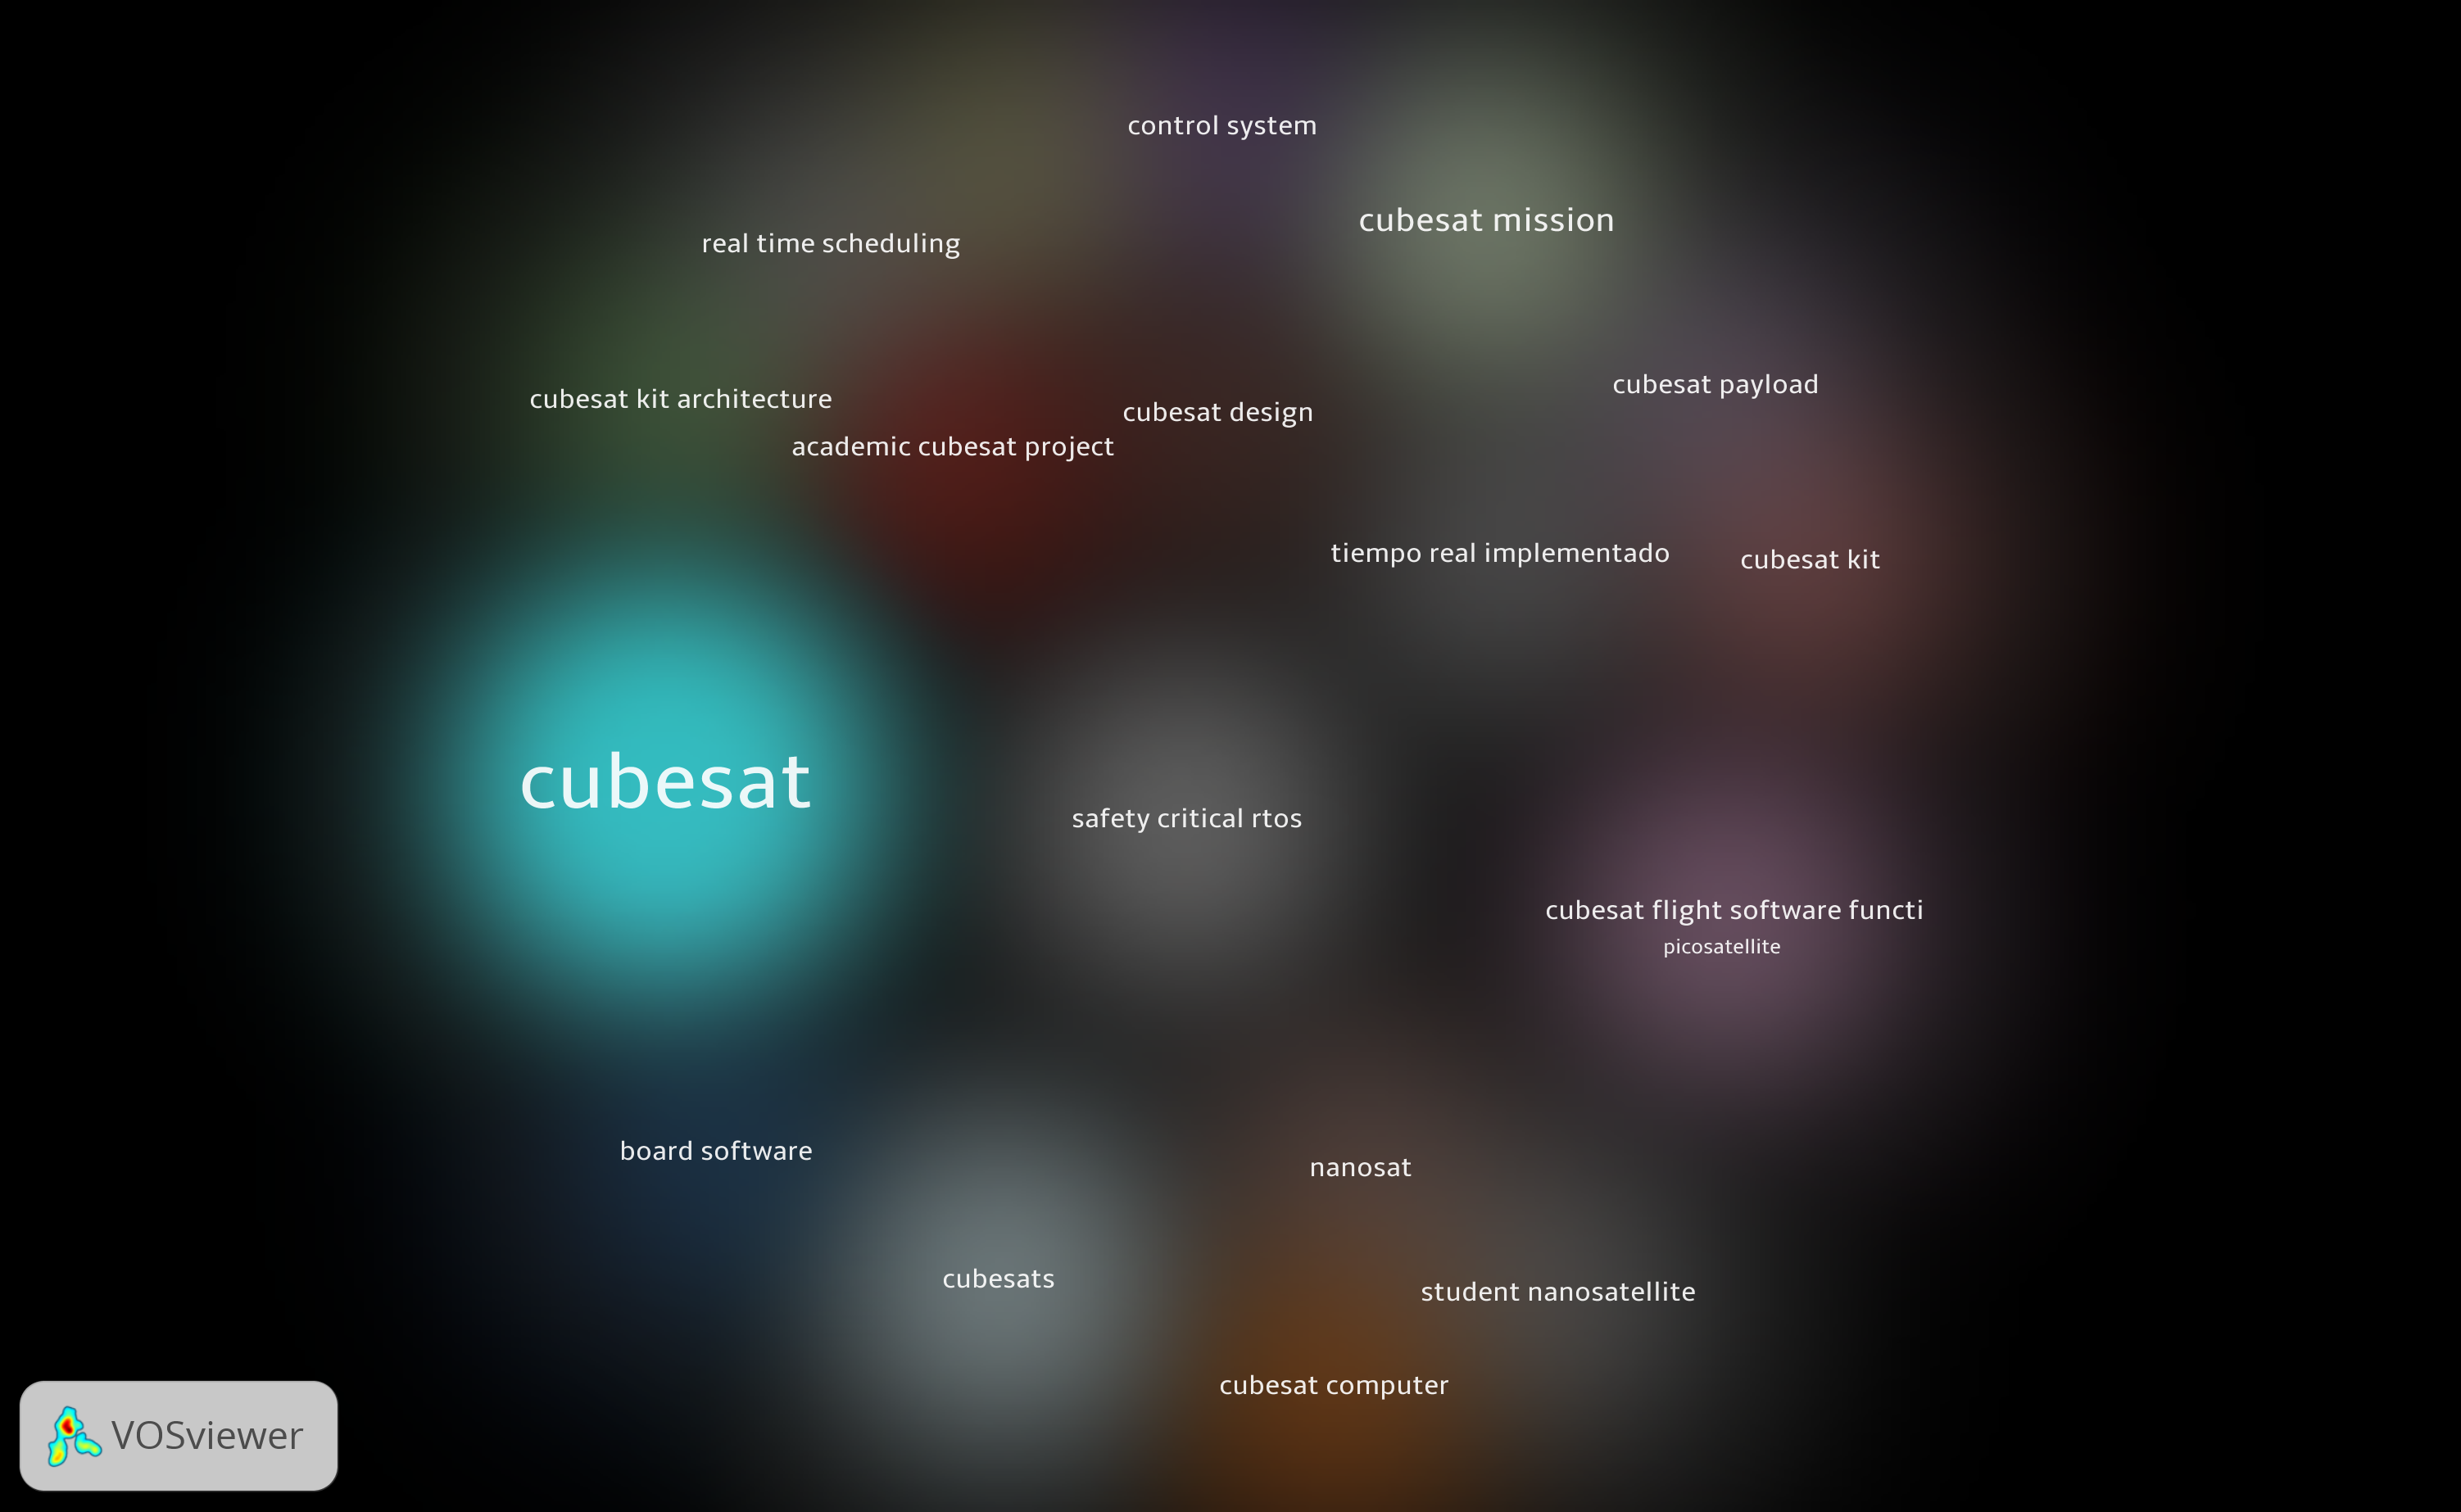
\includegraphics[width=15cm]{imagens/Cubesat_density_central.png}
	\caption{Mapa de visualização de densidade sobre o termo "Cubesat SO"}
	Fonte: Autor com base no Software VOSViwer.
	\label{fig: Cubesat Density Visualization}
\end{figure}

Ao redor do termo "cubesat", pode-se observar os termos correlacionado "academic cubesat project", 
"board software", "safety critical RTOS" e "cubesat kit architeture".Os cluster maiores e com cores mais 
vivas sinalizam um maior número de citações, a proximidade entre os termos indica correlação entre eles, 
todos os termos são encontrado sem trabalhos sobre cubesats, uma pesquisa na base de trabalhos Google 
Acadêmico retornou aproximadamente 16.900 resultados entre os anos de 2012 até 2021. Nota-se, na 
Figura~\ref{fig: Cubesat Published}, o número de trabalhos publicados por ano tem crescido a elevadas 
taxas anuais, chegando em 2020 com mais de 2.000 trabalhos publicados e citações contendo os termos 
"Cubesat SO" em título e resumo.


\begin{figure}[H]
	\centering
	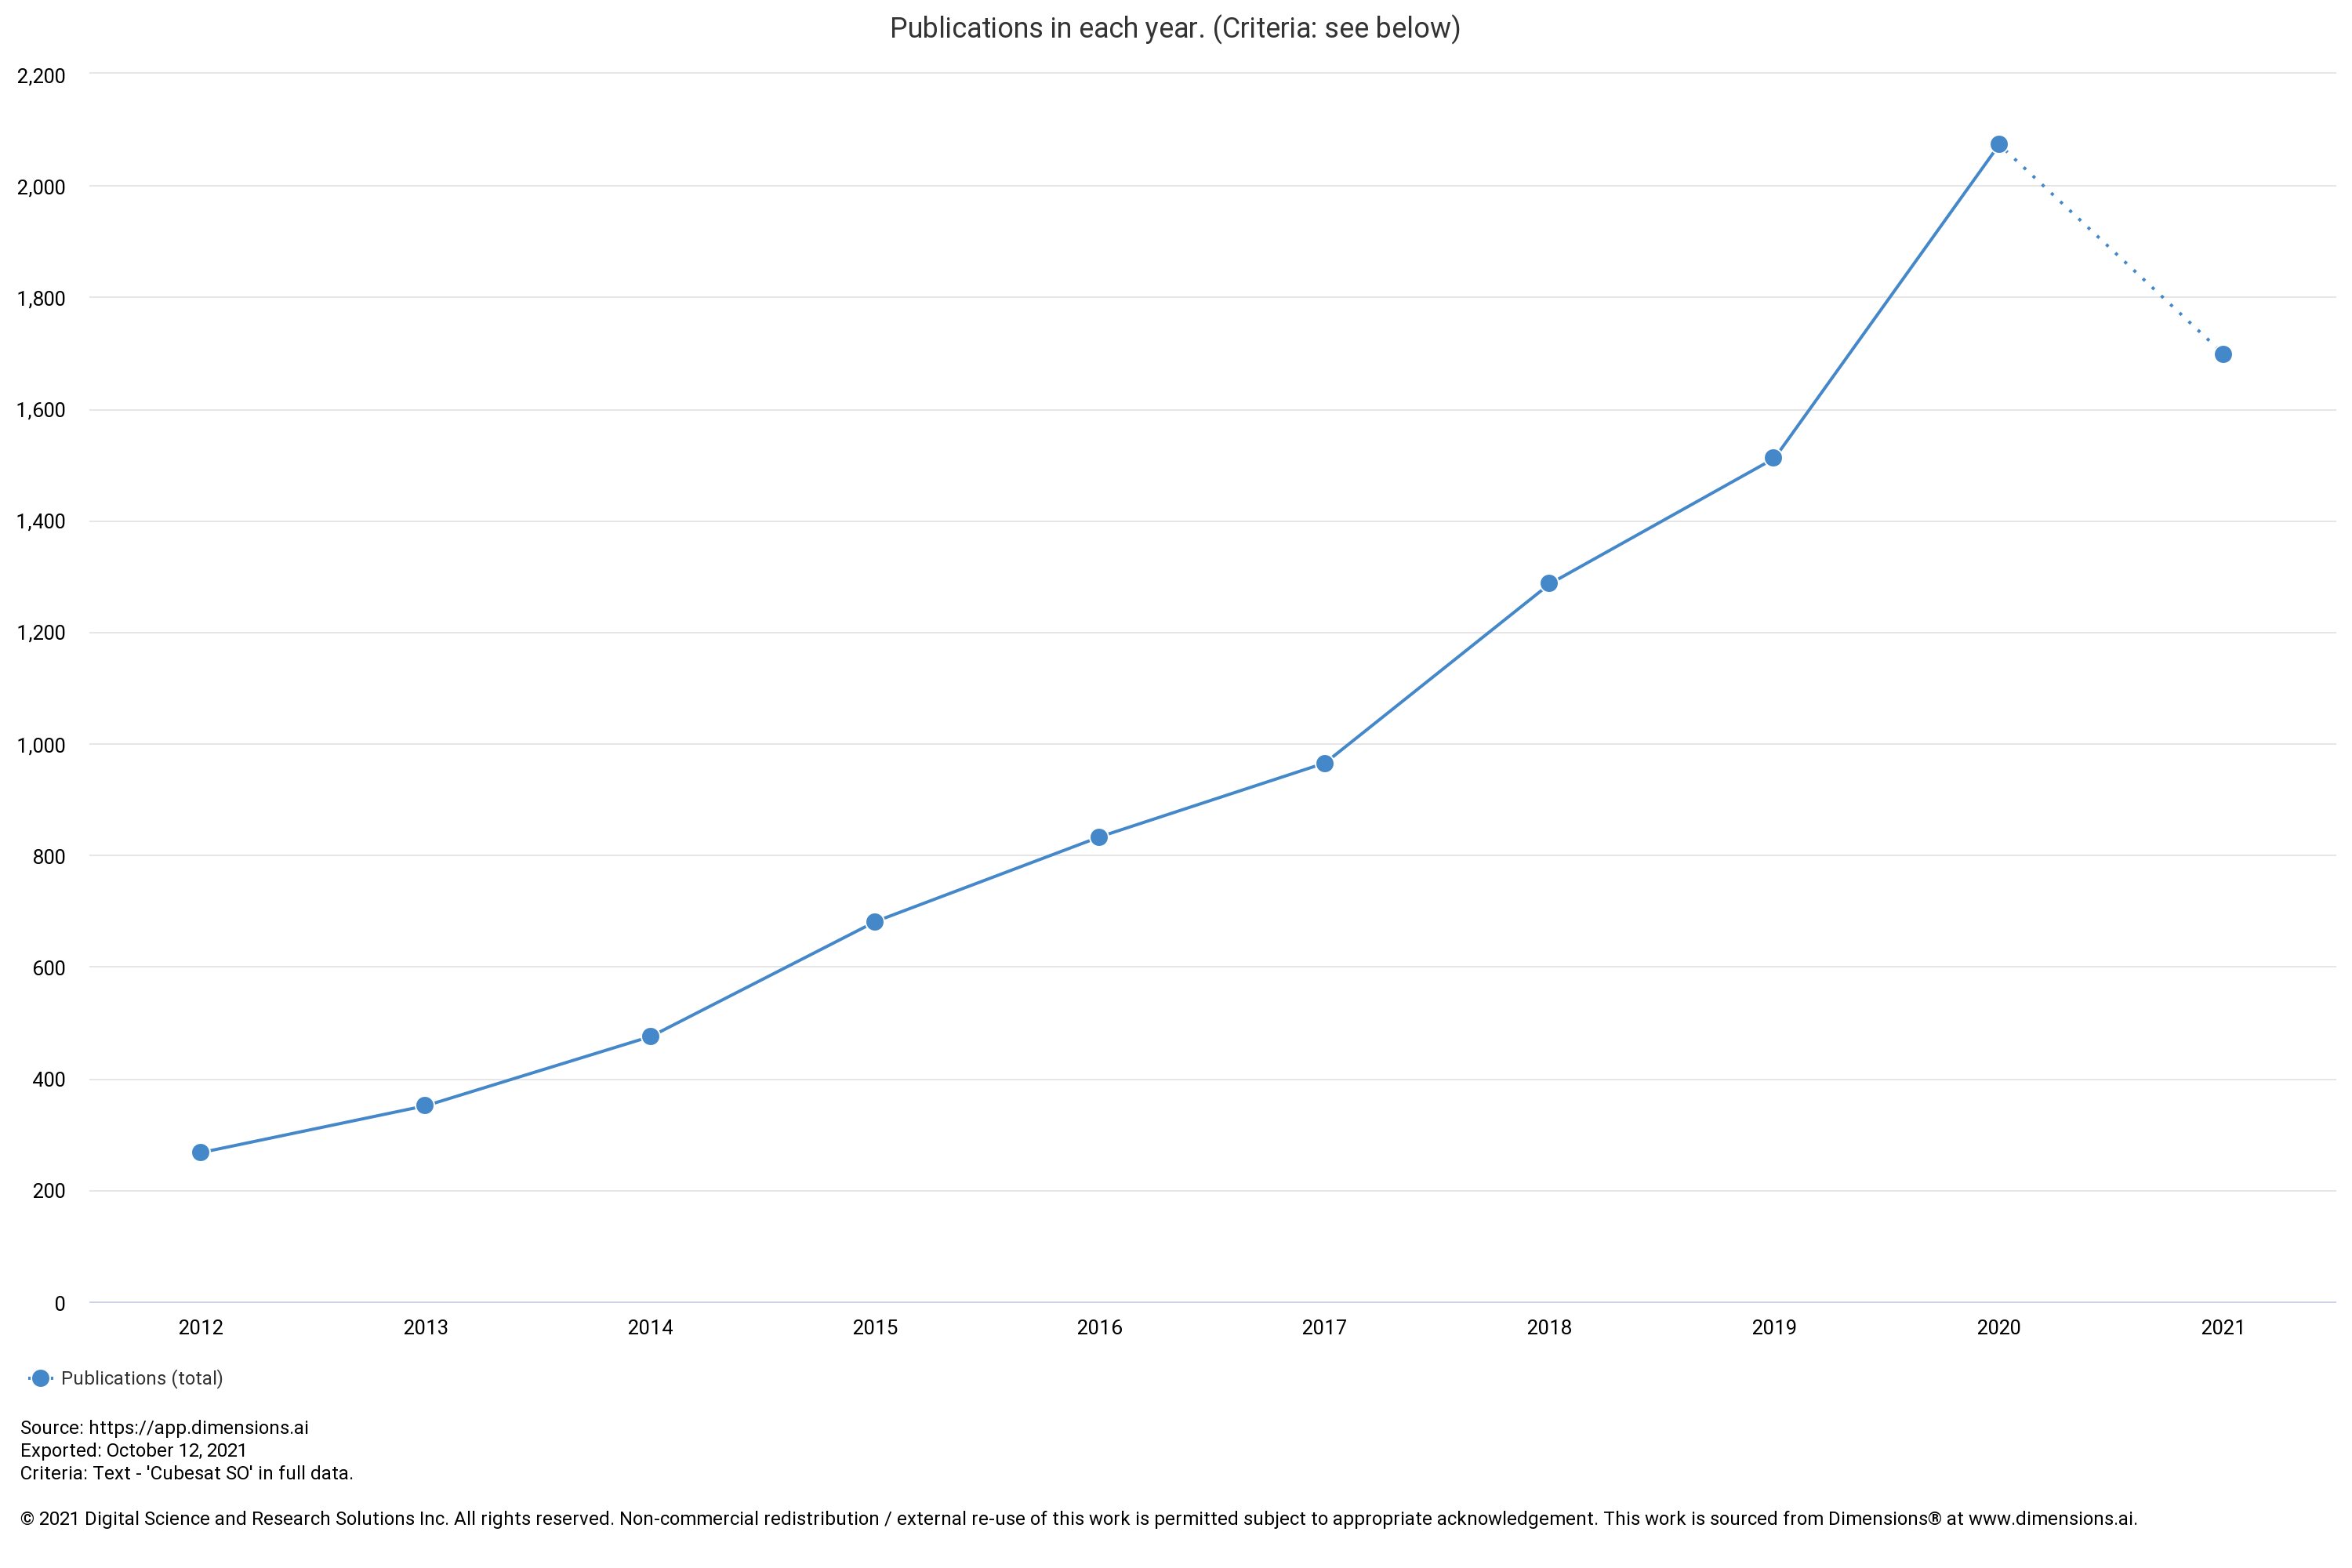
\includegraphics[width=15cm]{imagens/cubesat_publicados.png}
	\caption{A visualização mostra o número de publicações publicadas em cada ano de 2012 a 2021.}
	Fonte: Autor com base no site "dimensions.ai".
	\label{fig: Cubesat Published}
\end{figure}

Nota-se que o numero de trabalhos publicados e sempre maior que o ano anterior, reforçando a ideia de 
que os termos se encontram em destaque no meio acadêmico, com diversos trabalhos sendo correlacionados 
a iniciativas e nano satélites já concluídos ou em fase final de desenvolvimento. De acordo com \cite{Woellert2011} 
muitos destes projetos iniciam como spin-offs acadêmicos que terminam como uma atividade comercial.


\subsection{Conclusões sobre a Revisão Bibliométrica realizada}
% RTOS em CubeSats
Pode-se verificar a ocorrência de termos correlacionados nas duas pesquisas, com ênfase em 
"safety critical system" passando a ideia de conexão entre ambos, e interessante notar como 
os trabalhos sobre o projeto Zephyr tenta responder alguns dos problemas encontrados no 
desenvolvimento de um CubeSat, nota-se que o termo CubeSat e mais maduro do que o termo 
Zephyr, não encontrando nenhum trabalho relacionando os dois como um diferencial. 

% Ademais, 
% o levantamento bibliométrico passa a ideia que utilizar Zephyr em um projeto de Cubesat não 
% e uma ideia muito distante, abrindo uma janela de possíveis trabalhos na área que possam 
% trazer grandes contribuições, possibilitando o surgimento deste trabalho.

% Conclusão

% ---
% Capitulo de METODOLOGIA
% ---


\chapter{Metodologia}\label{cap:metodologia}
Nesta seção apresenta-se os materiais e métodos utilizados no desenvolvimento do trabalho proposto.
\section{Materiais e Métodos}

O presente estudo classifica-se como uma pesquisa experimental, a pesquisa experimental segundo \cite{wazlawick2017metodologia} condiciona o pesquisador a lidar com diversas variáveis experimentais e variáveis observacionais visando levar possivelmente, correlações e dependências entre as elas, utilizando de técnicas de amostragem e testes de hipóteses. O mesmo diz que trabalhos desenvolvidos em cima de abordagens padronizadas e aceitas internacionalmente, apresentando dados empíricos é relevantes, se encaixam no nível mais maduro de pesquisa, onde o autor deverá apresentar os resultados usando métricas aceitas pela comunidade, através de observações e medições, implicando que o pesquisador provocará alterações sistemáticas no ambiente do experimento para se observar os resultados após cada intervenção produzida.

\subsection{Materiais}

Para a implementação do método de intervalo de confiança, além da realização dos testes com dados em tempo real, utilizou-se dos seguintes materiais citados a seguir na tabela.

\begin{longtable}{|p{4cm}|p{3.5cm}|}
    \hiderowcolors
    \caption{Equipamentos utilizados}
    \label{tab:makespan}\\
    \showrowcolors
    \hline
    \rowcolor[HTML]{C0C0C0} 
    \multicolumn{1}{c|}{\cellcolor[HTML]{C0C0C0}\textbf{EQUIPAMENTO}} & \multicolumn{1}{c|}{\cellcolor[HTML]{C0C0C0}\textbf{UNIDADE}} \\ \hline

    \endfirsthead
    \rowcolor[HTML]{C0C0C0} 
    \multicolumn{1}{c|}{\cellcolor[HTML]{C0C0C0}\textbf{EQUIPAMENTO}} & \multicolumn{1}{c|}{\cellcolor[HTML]{C0C0C0}\textbf{UNIDADE}} \\ \hline

    \endhead
		\hline
		\textcolor[rgb]{0.125,0.129,0.141}{ESP32-DevKitC v1 ESP-WROOM-32U} & 1                \\
		\hline
		\textcolor[rgb]{0.059,0.067,0.067}{Cabo USB-Micro USB}          & 1                \\
		\hline
		Protoboard 400 pontos                                           & 1                \\
		\hline
		Sensor de temperatura termistor de 100k                         & 1                \\
		\hline
    
    \end{longtable}

O equipamento utilizado trata-se de um kit de desenvolvimento, apelidado de ESP32 DEV Kit v1 que acompanha o controlador ESP-WROOM-32, microprocessador Tensilica Xtensa 32-bit LX6 de dois cores, clock de até 240MHz, memória ROM de 448KB e SRAM de 520KB, e um termistor genérico de 100k que varia sua resistência dependendo da temperatura do ambiente retornando os dados para a análise.


\subsection{Análise exploratória dos dados}
Para avaliar o método de IC, foi necessário criar um conjunto de dados coletados através de um sensor de temperatura termistor de 100k acomodado no pino 21 do kit de desenvolvimento ESP32, aqui serão descritas as características mais importantes do dataset.

O conjunto contém 1592 linhas sem valores ausentes e 544 valores únicos com os valores \ang{32.14}c e \ang{33.47}c sendo os que mais se repetem com 35 aparições, todos os valores flutuando entre \ang{1.05}c e \ang{97.35}c graus, tendo média de \ang{37.19}c, desvio padrão de 13.33, primeiro quartil de 31.80, segundo quartil 33.00 e terceiro quartil em 35.33.
Os valores foram coletados no intervalo de aproximadamente 2 minutos, com todos os valores sendo processados na linguagem de programação Python na versão 3.11.0 com as bibliotecas pandas, numpy, matplotlib e scipy.


Na Figura~\ref{fig: hist} abaixo visualiza-se uma concentração maior de valores entre \ang{20}c e \ang{40}c graus com os valores seguintes podendo estar entre ruídos e picos de temperatura capturados pelo sensor. 

\begin{figure}[H]
	\centering
	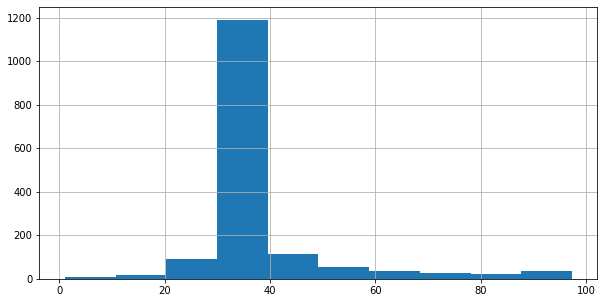
\includegraphics[width=15cm]{imagens/sensores/hist.png}
	\caption{histograma do conjunto de dados}
	Fonte: Autor com base na biblioteca pandas.
	\label{fig: hist}
\end{figure}

Tendo em vista que a média de temperatura do local de coleta da amostra estava entre \ang{33}c graus, pode-se visualizar uma grande quantidade de valores aproximados na Figura~\ref{fig: hist2}. 

\begin{figure}[H]
	\centering
	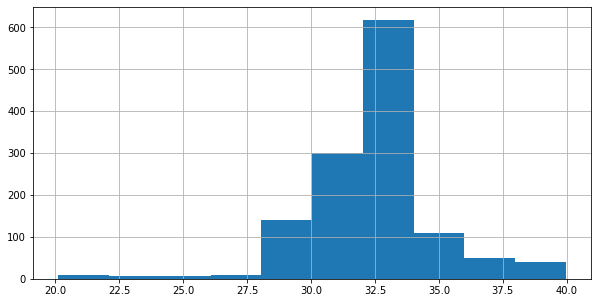
\includegraphics[width=15cm]{imagens/sensores/hist2.png}
	\caption{histograma do conjunto de dados entre 20 e 40 graus}
	Fonte: Autor com base na biblioteca pandas.
	\label{fig: hist2}
\end{figure}

\begin{figure}[H]
	\centering
	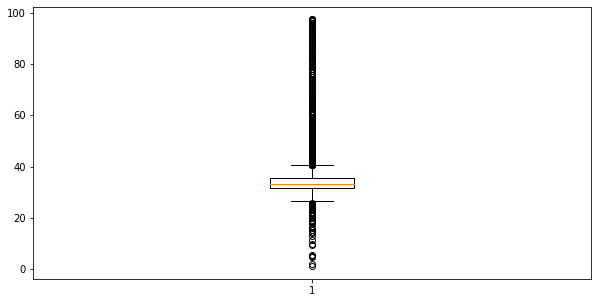
\includegraphics[width=15cm]{imagens/sensores/boxplot.png}
	\caption{Boxplot do conjunto de dados}
	Fonte: Autor com base na biblioteca matplotlib.
	\label{fig: boxplot}
\end{figure}

Verifica-se na Figuras~\ref{fig: boxplot} a grande presença de valores discrepantes acima de \ang{40}c e abaixo de \ang{20}c.

Abaixo na Figura~\ref{fig: bruto} pode-se visualizar todo o conjunto de dados, nota-se a presença de grandes picos de temperatura que foram induzidos na amostra propositalmente a fim de diferenciar o ruído do sensor de um pico de temperatura real, esses picos foram introduzidos através do aquecimento do sensor de temperatura duas vezes durante a coleta de dados.


\begin{figure}[H]
	\centering
	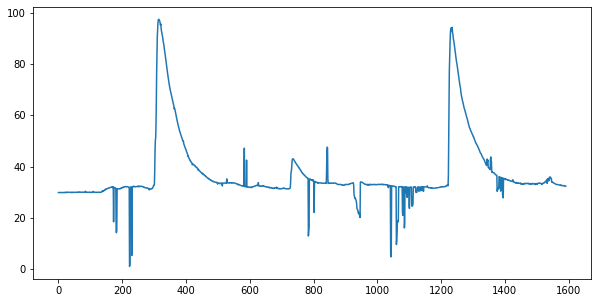
\includegraphics[width=15cm]{imagens/sensores/bruto.png}
	\caption{Plotagem gráfica do conjunto de dados completo}
	Fonte: Autor.
	\label{fig: bruto}
\end{figure}

As linhas verticais discrepantes indicam possíveis ruídos, onde a temperatura alcançou valores muito diferentes em períodos extremamente curtos. Esses ruídos podem ter sido gerados por baixa qualidade do termistor ou pela exposição ao ambiente dos fios de conexão entre o termistor e o microcontrolador.


\begin{figure}[H]
	\centering
	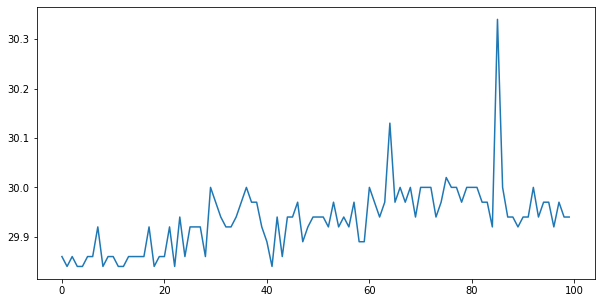
\includegraphics[width=15cm]{imagens/sensores/bruto_100_primeiras}
	\caption{Plotagem gráfica das 100 primeiras linhas do conjunto}
	Fonte: Autor.
	\label{fig: bruto_100p}
\end{figure}

Na Figura~\ref{fig: bruto_100p} percebe-se que a leitura do sensor sempre apresenta alguma variação, por mais pequena que seja, essa pequena diferença na coleta de dados pode não significar um problema, podendo ser tratada através de um simples cálculo de média. A criticidade dessa variação deve ser avaliada em cada projeto, com os dados ruidosos muito fora da média e esporádicos, interferindo significativamente no resultado final.

\begin{figure}[H]
	\centering
	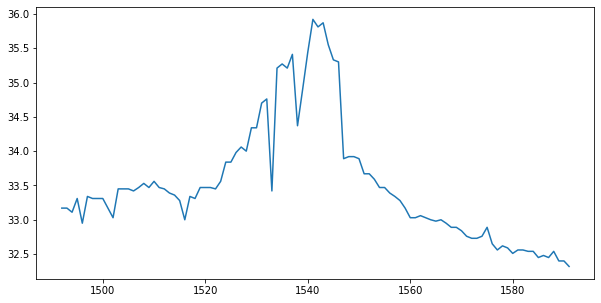
\includegraphics[width=15cm]{imagens/sensores/bruto_100_ultimas.png}
	\caption{Plotagem gráfica das 100 ultimas linhas do conjunto}
	Fonte: Autor.
	\label{fig: bruto_100u}
\end{figure}

Por fim na Figura~\ref{fig: bruto_100u} podemos analisar os últimos 100 dados, nos quais nota-se a presença de um pico de temperatura que começa a subir em \ang{33.05}c com sua máxima perto dos \ang{36.0}c, essa característica pode ser importante por mais que esteja em um curto período de tempo, e pode ser distinguida de um ruído pela sua característica de subida e descida prolongada. 




% % ---
% Capitulo de METODOLOGIA
% ---

\chapter{Definição de experimentos}\label{cap:definicoes}
\section{Introdução}
O experimento proposto neste trabalho seguirá da seguinte maneira, os testes serão
escritos na linguagem C nos dois RTOS escolhidos, ambos usarão funções iguais para
medida de tempo, cada teste terá seu arquivo individual para que não sofra
interferência de outros testes, todos serão disponibilizados na internet como código
aberto, afim que qualquer pessoa possa testar e validar os resultados aqui obtidos.

È muito importante que um sistema operacional de tempo real não deixe que tarefas
ocupem muito tempo para tomarem suas responsabilidades, isto impacta diretamente no
ciclo de toda a missão, tendo em vista que todo tempo e precioso para uma aplicação
que reaja quase em tempo real a qualquer situação. A medida de tempo será a subtração
do tempo de coleta inicial com o final, estas métricas são destinadas a oferecer
informações de tempo já que se supõe que o mesmo e muito importante para missões que
utilizem um RTOS.
% Definir o experimento
% Como vai ser feito
% Resultado esperado

\subsection{Velocidade de troca entre tarefas}
Durante o processo de encerramento de uma tarefa, o sistema operacional pode realizar
algumas operações, como vasculhar interrupções e quais as possíveis tarefas que
entrarão em seguida, tudo isso consome um tempo precioso para a aplicação
interferindo no tempo de troca para outra atividade, com o intuito de medir esse
tempo em milissegundos usaremos a função millis() para obter o tempo de troca entre
duas tarefas, subtraindo o tempo obtido no final da primeira tarefa e no começo da
segunda. Serão criadas duas tarefas,


%  Qual a politica de fila adotada?
uma com prioridade maior que a outra,


sendo a
com menor prioridade tendo a ação de despertar a outra, o tempo que leva para a outra
tarefa ser despertada será medido. Espera-se que a troca entre as tarefas seja a mais
rápida possível, não apresentando gargalos, e que a tarefa com menor prioridade consiga
despertar a outra tarefa, mesmo que seja de prioridade maior.

\subsection{Tempo de passagem de mensagens entre tarefas}
É muito importante que as tarefas possam se comunicar entre si, de preferência de
forma mais rápida possível evitando que se encontrem bloqueadas esperando alguma
resposta, o tempo de envio e recebimento será medido tendo entre tarefas com prioridades
iguais, quanto entre tarefas de prioridades diferentes, espera-se que o sistema evite
bloqueios após a solicitação de envio em uma mensagens. Durante uma missão as tarefas
trocaram muitas mensagens, já que muito da operação depende que os módulos do satélite
troquem informações entre si, a troca destas mensagens não pode prejudicar o andamento
de todo o sistema.

\subsection{Tempo de bloqueio e liberação de desbloqueio de Semáforo e Mutex}
Iremos medir o tempo que o RTOS leva para bloquear um Semáforo e Mutex, junto também
o tempo para liberação, este teste necessita apenas de uma tarefa, a qual solicita e
libera em seguida o semáforo ou mutex. È importante que este tempo seja o mais curto
possível, já que outras tarefas também podem depender desta mesma variável, sendo o
tempo de liberação mais importante. Durante uma missão varias

% Que tipo de operações serão realizadas?
tarefas

pediram permissão
para usar o mesmo recurso, sendo que o controle de acesso para evitar possíveis
conflitos responsabilidade dos Semáforos e Mutexes, pouco atraso na troca destes pode
ocasionar em possíveis problemas de prioridades, levando com que tarefas com prioridades
maiores levem mais tempo para conseguirem liberação.

\subsection{Tempo de resposta a eventos externos atraves de interrupção}
Durante uma missão o sistema lidara com diversas interrupções, sendo elas de alta
prioridade e devendo serem tratadas imediatamente, este teste esta muito
correlacionado com o primeiro, já que iremos medir o tempo que leva para uma tarefa
despertar através desta vez por uma

% Como será implementado essa rotina?
rotina de interrupção.

O controlador da missão
terá que lidar com diversas ISR durante a missão, sendo importante que nenhuma delas
fique para trás ou que atrapalhem o ciclo de vida do sistema.

\subsection{Velocidade de alocação de memoria}
Alocar memória para realizar alguma operação pode levar algum tempo, todo RTOS tem
suas funções para alocação de memória, e cabe a este teste coletar medida de tempo
nesta operação, seja qual for o tamanho de memória requisitada o sistema deve
entrega-la rapidamente, aqui selecionaremos uma região de memória RAM e o tempo para
aquisição e liberação da mesma será medida. Aqui se destaca cada RTOS com suas regras
de alocação de blocos de memória, poderemos notar qual a diferença das abordagens e se
adequam nas operações rápidas de uma tarefa.

\subsection{Velocidade de leitura e gravação em memoria flash (Cartão SD)}
Este teste é muito semelhante ao anterior, mas se difere por utilizar de memória flash,
aqui mais especifico duas memórias, já que faremos testes alocando memoria flash
internado ESP32 como também um cartão SD externo. Em muitas missões de CubeSat memoria
flash externas são usadas como backup do sistema entre outras aplicações como
armazenamentos de dados científicos antes do seu envio para a terra. Espera-se que
esta operação seja rápida e não corrompida, já que o envio destes dados e crucial para
o objetivo final da missão.

\chapter{Resultados}\label{cap:resultados}
\section{Introdução}






\chapter{Conclusão}\label{cap:conclusao}

Os sensores fazem parte da revolução tecnológica que o mundo tem passado, os dados coletados pelos mesmos são utilizados nas mais diversas esferas, são relevantes para as tomadas de decisão e estão sempre sujeitos a interferências.
 
Espera-se que todo sinal vindo de qualquer sensor esteja com algum ruído, e que sejam tratados de alguma forma. Para isso existem diversas funções para se retirar valores discrepantes, muitas delas interferem na forma do sinal real tratando o dado e retirando um novo valor resultante e de maior precisão, essa ação pode ser prejudicial em muitos dos casos alterando o real valor e dificultando ou atrasando a visualização de mudanças bruscas, muito importantes em algumas analise de dados. No ambiente de sistemas embarcados é muito importante que qualquer algoritmo respeite as limitações de memória, processamento e tempo. Algumas funções podem exigir muito processamento ou até mesmo muita memória para realizar todos os cálculos responsáveis pela filtragem, com esse problema é importante que a função esteja dentro dos parâmetros para trabalhar em ambiente restrito.
Este trabalho teve como objetivo apresentar o desvio de confiança como uma boa alternativa para ser utilizada como filtro em ambiente embarcado, além disso é importante que os dados filtrados permaneçam os mais originais possíveis. 
O resultado encontrado com o algoritmo proposto é capaz de manipular um vetor de amostra móvel com eficácia, além de manter os dados de forma original mas com o crivo dos valores dentro de um intervalo aceitável de confiança. Mas observou-se problemas importantes, como não conseguir registrar sinais em curvas muito prolongadas, o que tornava a espera por um novo sinal confiável muito longa e atrapalhava o andamento do programa, por mais que o algoritmo tenha se saído bem em retornar os valores superiores de todos os picos de valores. Também notou-se que os dados resultantes por serem intocáveis, entregavam a possibilidade do método ser utilizado em conjunto com outros que posteriormente coletariam os dados, filtrando-os em busca de valores mais amenizados dependendo da aplicação.
 
O tempo envolvido neste trabalho não foi o suficiente para a realização de todos os cálculos em linguagem C em um sistema embarcado, mas o tratamento provou-se ser viável e poderia ser aplicado em conjunto com outros métodos em trabalhos futuros. Retornando à comunidade de desenvolvimento de filtros digitais em sistemas embarcados uma alternativa aberta a ser utilizada.


\section{Trabalhos Futuros}

\begin{itemize}
    \item Utilizar o filtro apresentado com outras funções de filtragem.
    \item Escrever o filtro em uma aplicação real de coleta de dados.
  \end{itemize}



% ----------------------------------------------------------
% ELEMENTOS PÓS-TEXTUAIS
% ----------------------------------------------------------
\postextual
% ----------------------------------------------------------

% ----------------------------------------------------------
% Referências bibliográficas
% ----------------------------------------------------------
%\bibliography{bibliografia}
\bibliography{bibliografia}
% ----------------------------------------------------------
% Glossário
% ----------------------------------------------------------
%
% Consulte o manual da classe abntex2 para orientações sobre o glossário.
%
%\glossary

%---------------------------------------------------------------------
% INDICE REMISSIVO
%---------------------------------------------------------------------
\phantompart
\printindex
%---------------------------------------------------------------------

\end{document}
\grid
